\section{Data Analysis}
\label{sec:Data Analyses}

This study utilizes data from the ASHRAE Great Energy Predictor III Kaggle competition \cite{ashrae-energy-prediction}, a significant data science challenge focused on developing accurate building energy consumption prediction models. The competition provided a comprehensive dataset designed to forecast metered building energy usage across four energy types, with data collected from over 1,000 buildings.

\subsection{Dataset Description}

The original dataset consists of several interconnected files, each serving a specific purpose in the energy prediction task. The primary file, train\.csv, contains historical meter readings with essential columns including building\_id as a foreign key to building metadata, meter type indicators (0 for electricity, 1 for chilled water, 2 for steam, and 3 for hot water), timestamp information for each reading, and the target variable meter\_reading representing actual energy consumption. Complementing this is test\.csv which follows an identical structure but omits the meter\_reading values.

Building characteristics are stored in building\_metadata\.csv, which provides static information about each building. This file includes unique building identifiers, site location codes, primary use categorization (such as education, office, parks or healthcare facilities), square footage information, construction year, and floor count. These attributes provide context for understanding energy consumption patterns across different building types and configurations.

Weather conditions, which significantly influence energy usage, are contained in weather\_train\.csv and weather\_test\.csv for the training and testing periods respectively. These files include site-specific weather measurements captured at regular intervals, featuring air temperature in Celsius, cloud coverage measured in oktas, dew point temperature in Celsius, hourly precipitation depth in millimeters, sea level pressure in millibars, wind direction in degrees, and wind speed in meters per second. This comprehensive weather data enables models to account for environmental factors when predicting energy consumption.


\subsection{Data Pre-Processing}

The data transformation process began with a comprehensive integration of the five CSV files from the original dataset. First, we established relational connections between these files to create a unified analytical base. Initially, building\_metadata\.csv was joined with train\.csv using the building\_id column as the linking key, enriching energy consumption data with building characteristics. Afterward, weather conditions from weather\_train\.csv were incorporated using site\_id and timestamp columns to align environmental factors with corresponding energy readings. 

Following integration, we implemented a filtering criteria to focus exclusively on electricity consumption. By retaining only records where meter = 0, we significantly reduced the dataset size from approximately 20 million to 12 million rows, creating a more focused and manageable dataset while maintaining sufficient data volume for robust analysis. In addition to this filtering, we removed columns demonstrating low predictive power for electricity consumption based on correlation analysis, specifically wind\_direction (correlation: 0.04), wind\_speed (correlation: 0.08), and sea\_level\_pressure (correlation: 0.03), concentrating only on features with demonstrated relevance to electricity consumption prediction.

The dataset contained various patterns of missing values requiring systematic treatment. Weather-related features showed temporal gaps, with air\_temperature missing 4.8\% of values, cloud\_coverage missing 12.3\%, dew\_temperature missing 5.1\%, and precip\_depth\_1\_hr missing 6.7\%. To address these gaps while preserving data characteristics, we implemented a two-step imputation approach: first replacing missing values with the median value for the same site\_id, then filling any remaining missing values with the global median. This methodology preserved site-specific weather patterns while ensuring dataset completeness without introducing artificial anomalies.

Building metadata presented more significant completeness challenges, with year\_built missing in 25.8\% of records and floor\_count absent in 18.4\%. After careful consideration of various approaches, we chose to remove buildings with missing metadata rather than attempt imputation. This decision was based on several key factors: these static, structural features could introduce significant bias if imputed incorrectly; the values are not time-dependent and cannot be reasonably estimated from nearby readings; and even after removal, we retained a sufficiently large dataset (2 million rows) to support robust analysis. This choice prioritized data quality over quantity, reducing the dataset from 12 million to 2 million rows but ensuring higher reliability in the retained data.

To validate our feature selection decisions, we conducted a comprehensive correlation analysis between all potential predictors and electricity consumption. The results confirmed the importance of air\_temperature (0.68 correlation) and square\_feet (0.65 correlation) as primary predictors, with dew\_temperature (0.52), cloud\_coverage (0.23), and precip\_depth\_1\_hr (0.11) also showing meaningful relationships. Based on this analysis, we retained features with correlations above 0.10 and removed others with weaker relationships, as already mentioned before.


\subsection{Data Processing and Data Visualization}

To begin the modeling process, we conducted a thorough pre-processing pipeline that involved cleaning, filtering, engineering new features, and transforming the dataset to ensure quality and consistency.

\subsubsection{Data Cleaning}


We began by converting the timestamp column to datetime format, enabling time-series analysis crucial for energy consumption patterns.

Next, we evaluated the completeness of observations per building. Since the dataset spans hourly readings across an entire year (i.e., 365 days * 24 hours), we expected 8,760 observations per building. However, some buildings had significant gaps, with entire days missing.

\begin{figure}[!h]
    \centering
    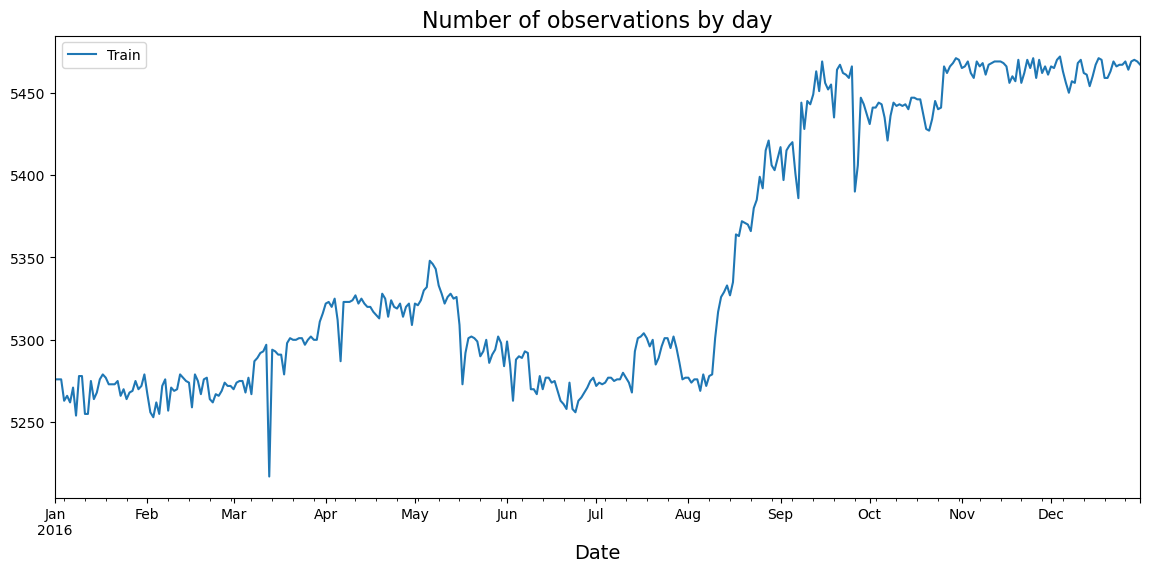
\includegraphics[width=0.75\linewidth]{images/obser_by_day.png}
    \caption{Observations per month with failures}
    \label{fig:obs-by-month-bad}
\end{figure}

To maintain data integrity, we removed buildings with missing target values for entire days, retaining approximately 130 buildings with consistent readings, Fig. \ref{fig:obs-by-month-good}. This resulted in a dataset with around 3,000 observations per day, totaling over one million rows. We then reindexed the dataset to include all combinations of building\_id and timestamp for the year 2016, ensuring temporal continuity.

\begin{figure}[!h]
    \centering
    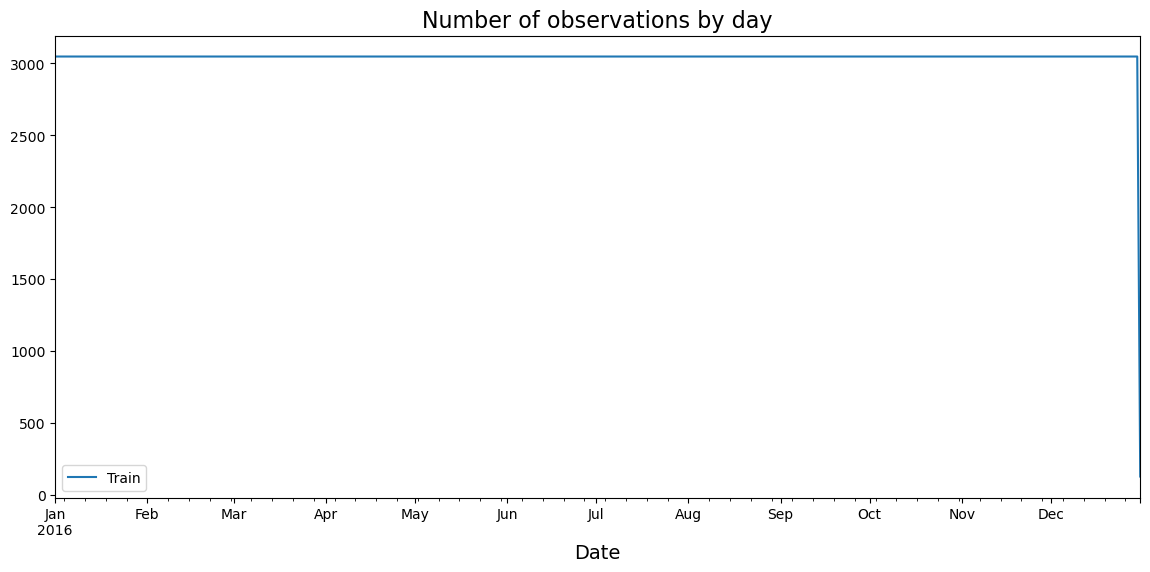
\includegraphics[width=0.75\linewidth]{images/obser-good.png}
    \caption{Observations per month}
    \label{fig:obs-by-month-good}
\end{figure}

We then analyzed the distribution of buildings across the primary\_use categories, Fig. \ref{fig:primary_use_before_delete}. To ensure statistical robustness and avoid sparsity issues, we excluded categories with fewer than 10 unique buildings ('Other', 'Healthcare', 'Manufacturing/industrial'). 

\begin{figure}[!h]
    \centering
    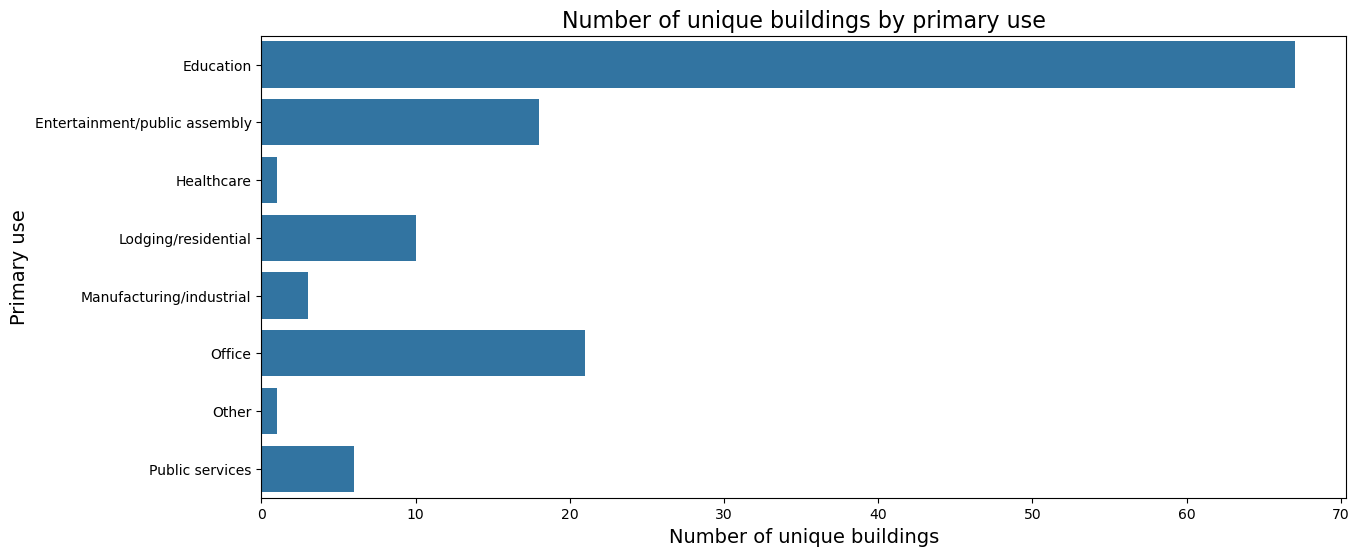
\includegraphics[width=0.75\linewidth]{images/primary_use_after_deleting.png}
    \caption{Number of Unique buildings by Primary Use}
    \label{fig:primary_use_before_delete}
\end{figure}

After this filtering, we performed targeted analysis of the target variable across categories. For instance, we observed that schools and offices had noticeably higher energy consumption, reflecting their more intensive operational schedules, Fig. \ref{fig:energy_consu_by_primary_use}.

\begin{figure}[!h]
    \centering
    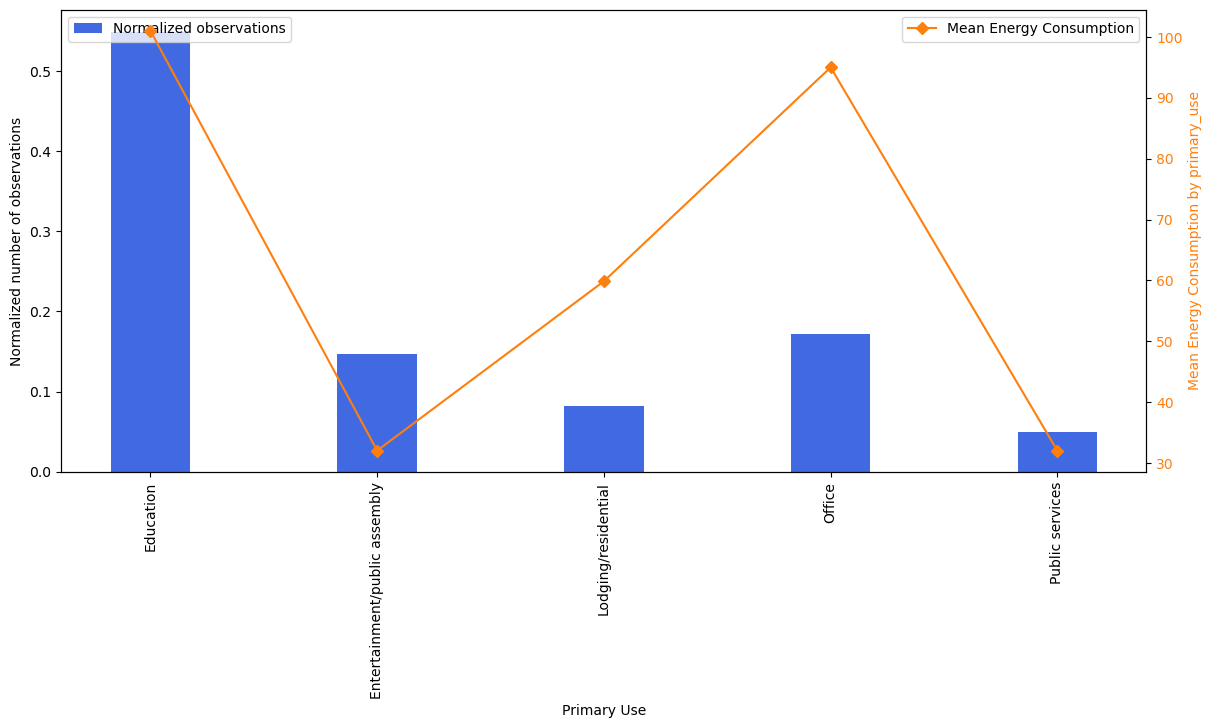
\includegraphics[width=0.75\linewidth]{images/energy_consu_by_primary_use.png}
    \caption{Energy Consumption by primary\_use}
    \label{fig:energy_consu_by_primary_use}
\end{figure}

After, we started by examining the target variable (energy consumption), Fig. \ref{fig:energy_consu_by_site} and air temperature, Fig. \ref{fig:temp_by_site}across different site\_ids. The goal was to assess whether temporal patterns. This preliminary analysis revealed that although some variation existed, the overall structure was sufficiently aligned, allowing for a unified modeling approach across locations.

\begin{figure}[!h]
    \centering
    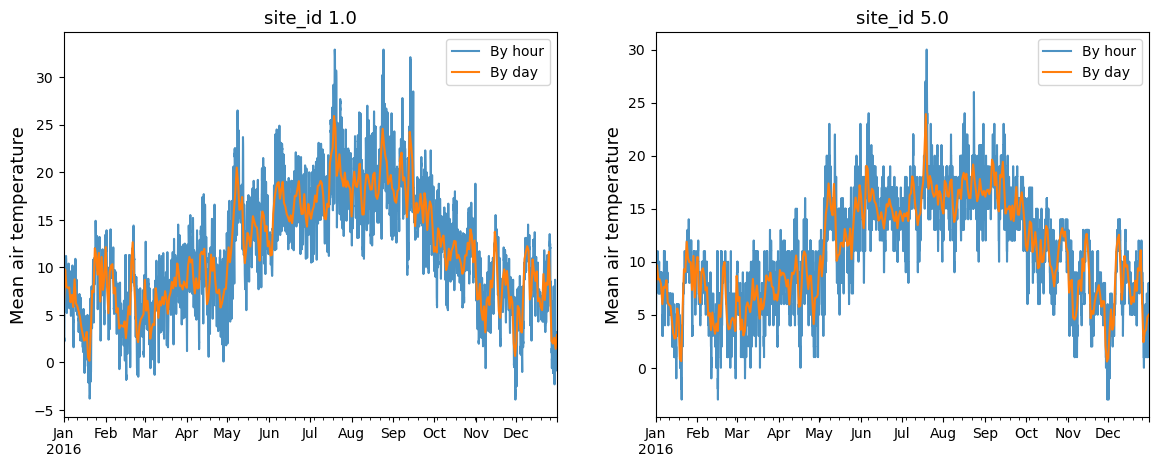
\includegraphics[width=\linewidth]{images/temperature-by-site.png}
    \caption{Air Temperature by Site}
    \label{fig:temp_by_site}
\end{figure}
\begin{figure}[!h]
    \centering
    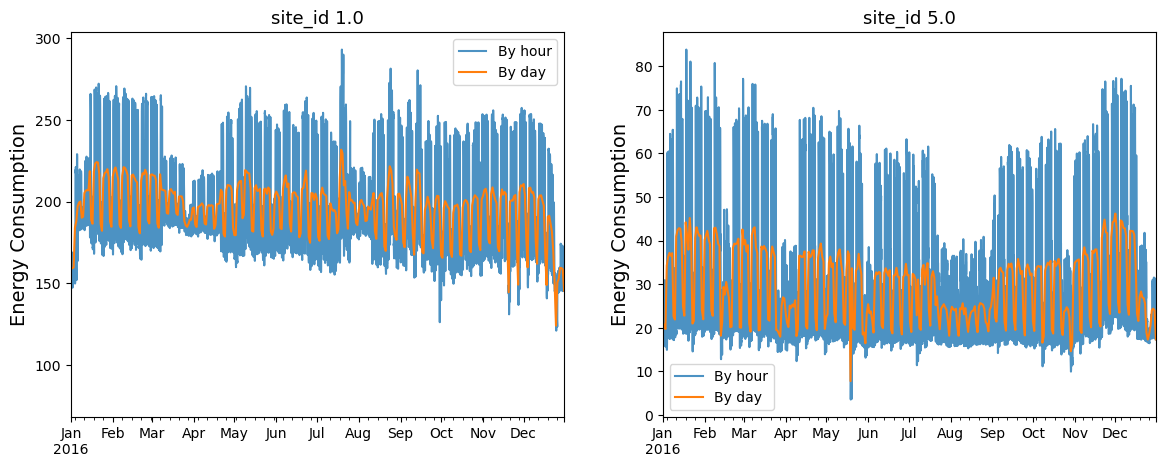
\includegraphics[width=1\linewidth]{images/energy-by-id.png}
    \caption{Energy Consumption by Site}
    \label{fig:energy_consu_by_site}
\end{figure}

\subsubsection{Feature Engineering}
Following the cleaning phase, we moved into feature engineering. We extracted key time-based features from the timestamp column, including hour, day, weekday, and month, to capture daily, weekly, and seasonal consumption cycles. Additionally, we created a new feature, m2\_per\_floor, computed as the ratio between square\_feet and floor\_count, to represent the average area per floor — a potentially useful indicator of spatial density and building efficiency.

Categorical variables required special attention, particularly primary\_use which classifies buildings into functional categories. We applied OneHotEncoder to transform these categorical values into binary representations suitable for machine learning algorithms. This approach preserves the categorical information while avoiding arbitrary ordinal relationships between different building types.

We also engineered a set of lag features for both the target (energy consumption) and air\_temperature, using time lags of 1, 6, 12, 72 (3 days), 120 (5 days), and 168 hours (7 days). These features are essential for capturing temporal dependencies and autoregressive patterns.

\subsubsection{Data Transformation}

\begin{figure}[!h]
    \centering
    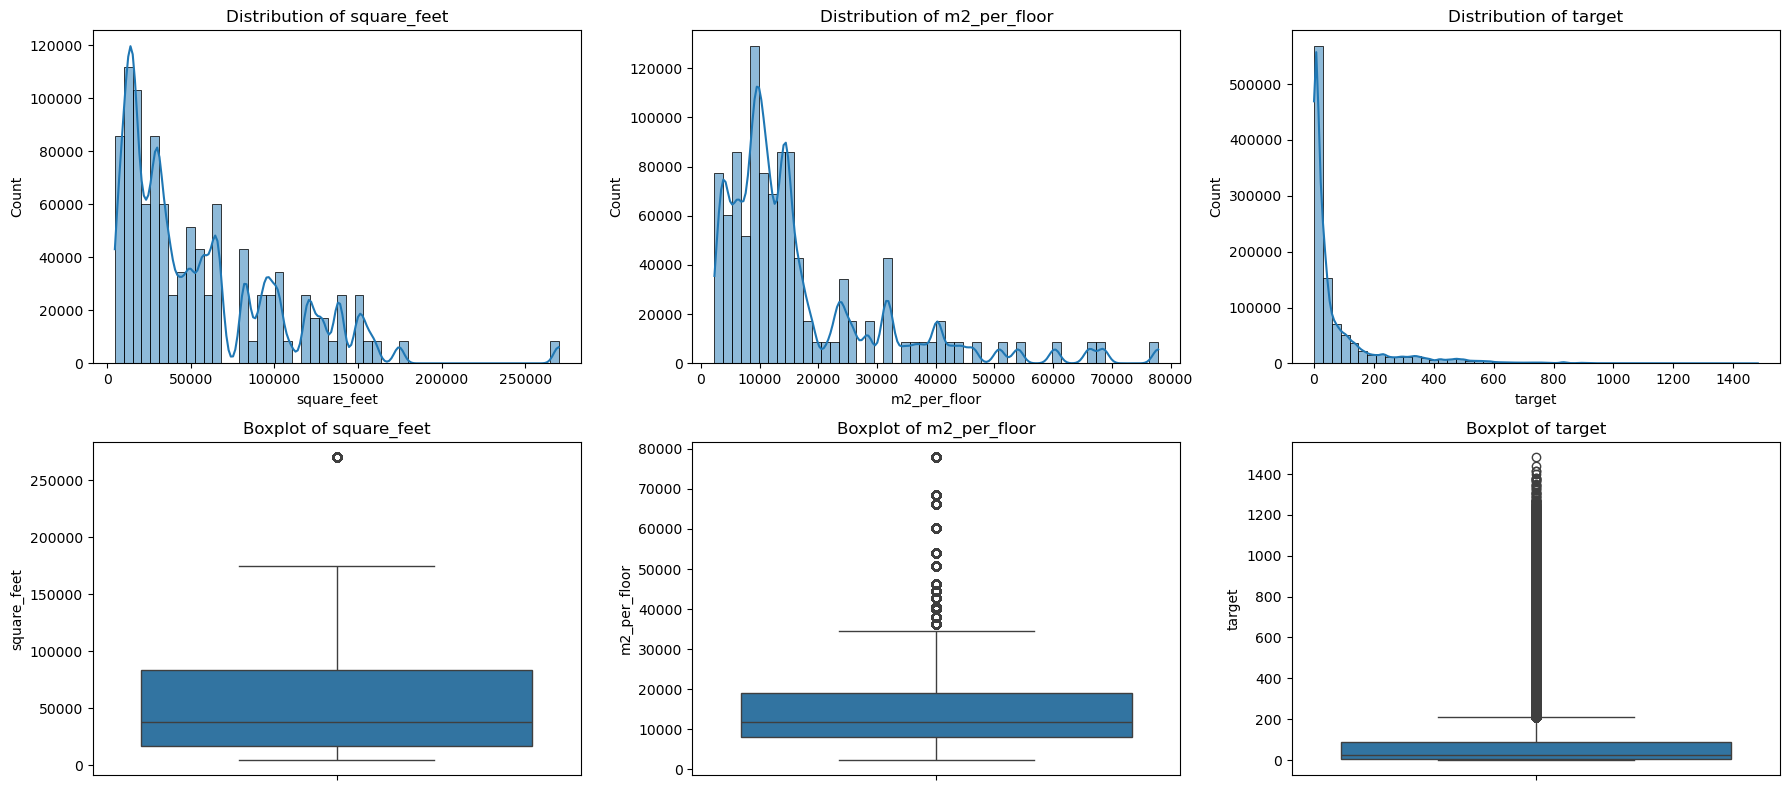
\includegraphics[width=1\linewidth]{images/non-distrib.png}
    \caption{Variables Distributions Before Logarithmic Transformation}
    \label{fig:non-label}
\end{figure}
To address the non-normal distributions evident in Figure \ref{fig:non-label}, we applied logarithmic transformations to several numerical features, including square\_feet, m2\_per\_floor, and the target variable. This transformation effectively compressed the range of large values and expanded the range of small values, resulting in more symmetric distributions that better satisfy the assumptions of many machine learning algorithms, as demonstrated in Figure \ref{fig:Variables Distributions After Logarithmic Transformation}.


\begin{figure}[!h]
\centering
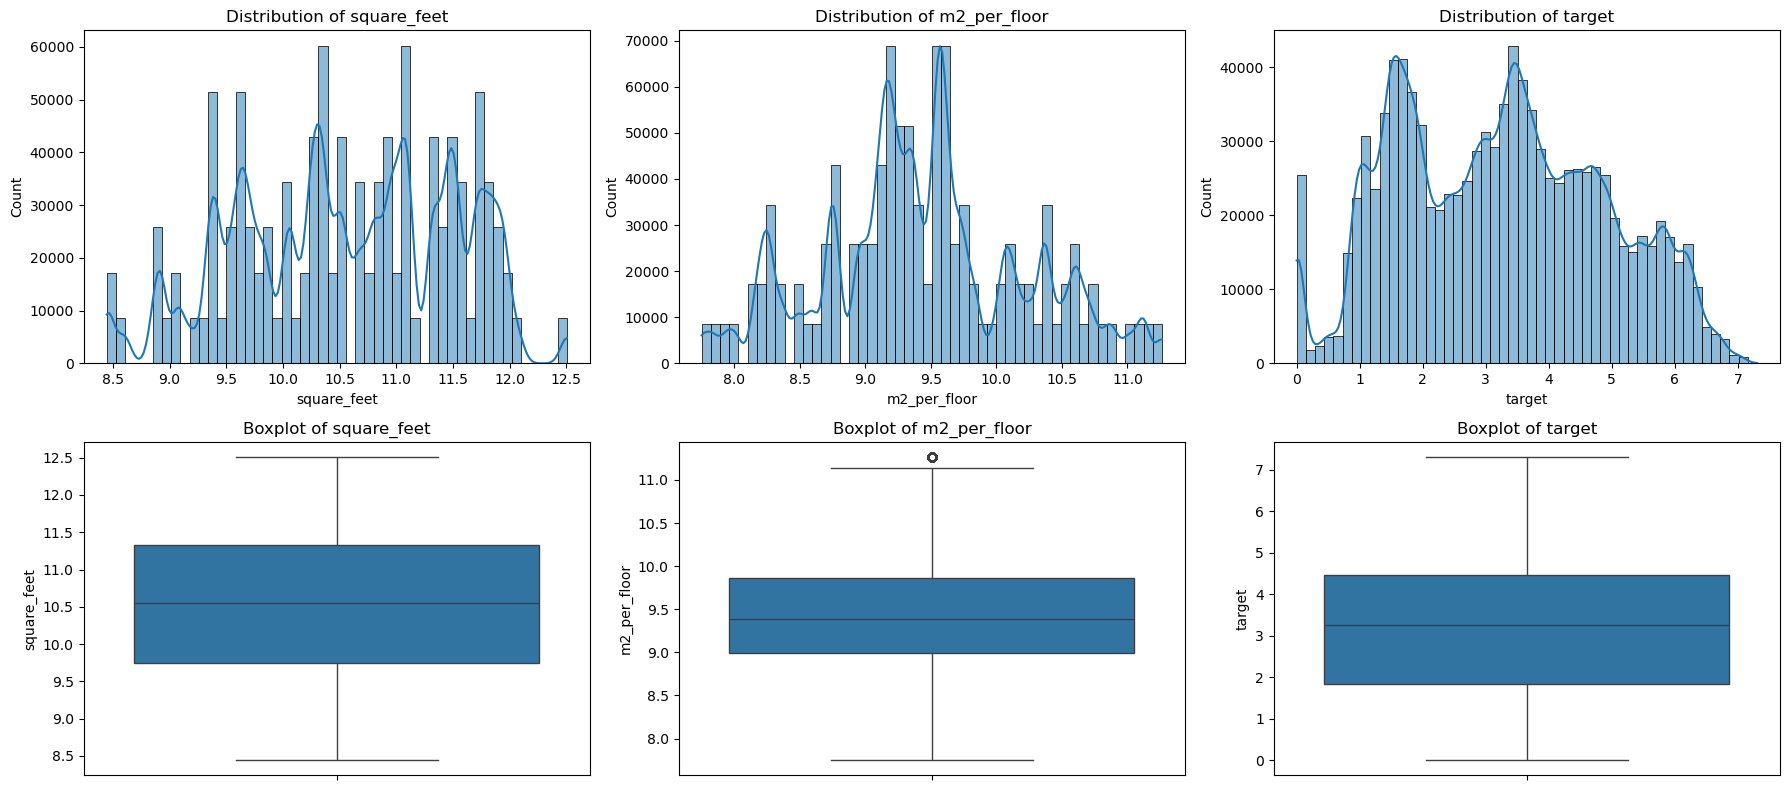
\includegraphics[width=1\linewidth]{images/box_plot-destribution.png}
\caption{Variables Distributions After Logarithmic Transformation}
\label{fig:Variables Distributions After Logarithmic Transformation}
\end{figure}

\begin{figure}[!h]
    \centering
    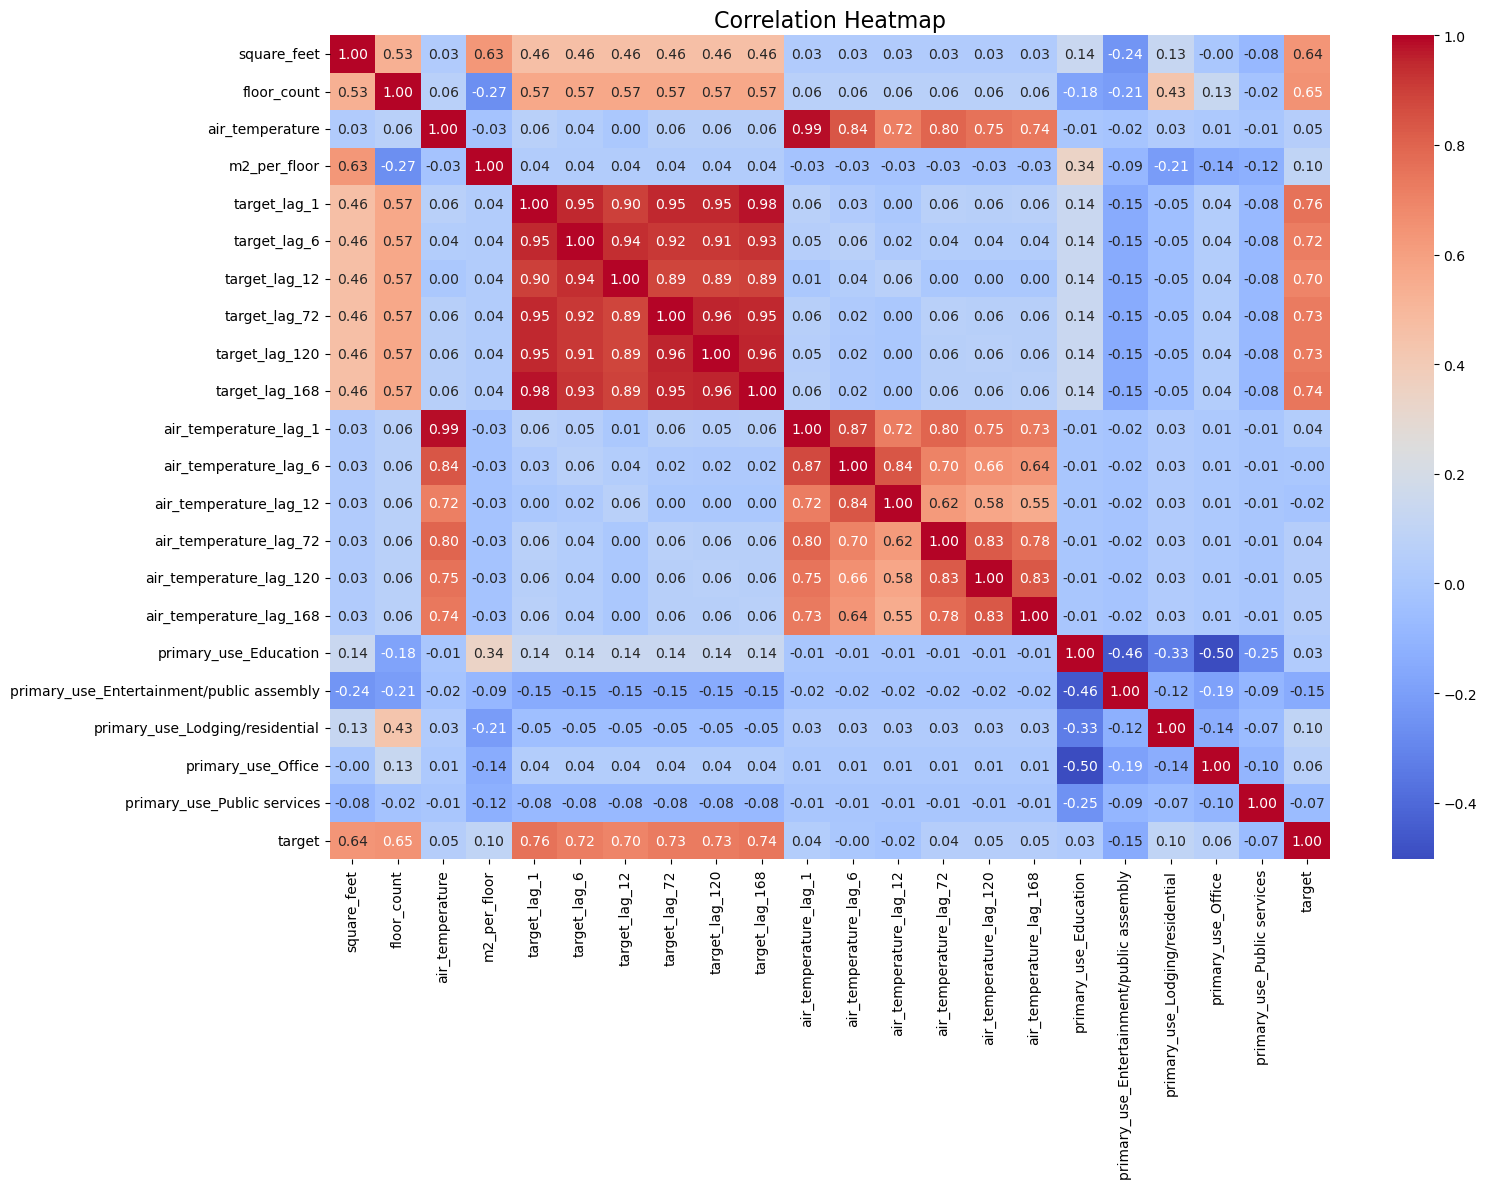
\includegraphics[width=1\linewidth]{images/corr_matrix.png}
    \caption{Correlation Matrix}
    \label{fig:enter-label}
\end{figure}

After feature engineering, we assessed feature importance through correlation analysis and removed variables showing minimal correlation with the target, streamlining the model input space without sacrificing predictive power.


Table \ref{tab:feature_descriptions} presents the complete set of features used in our analysis after preprocessing.

\begin{table}[!h]
\centering
\caption{Feature Descriptions}
\label{tab:feature_descriptions}
\begin{tabular}{|>{\raggedright\arraybackslash}p{2cm}|>{\raggedright\arraybackslash}p{5cm}|}
\hline
\textbf{Feature Name} & \textbf{Feature Description} \\
\hline
\texttt{primary\_use} & The primary functional category of the building (e.g., Education, Office). This feature was one-hot encoded. \\
\texttt{square feet} & Total area of the building in square feet (log-transformed). \\
\texttt{year built} & Year the building was constructed. \\
\texttt{floor count} & Number of floors in the building. \\
\texttt{air temperature} & Hourly air temperature in degrees Celsius. \\
\texttt{m2\_per\_floor} & Average square meters per floor (log-transformed). \\
\texttt{target} & Energy consumption in kilowatt-hours (kWh), measured hourly (log-transformed). \\
\texttt{target\_lag\_1} & Energy consumption 1 hour prior. \\
\texttt{target\_lag\_6} & Energy consumption 6 hours prior. \\
\texttt{target\_lag\_12} & Energy consumption 12 hours prior. \\
\texttt{target\_lag\_72} & Energy consumption 3 days prior. \\
\texttt{target\_lag\_120} & Energy consumption 5 days prior. \\
\texttt{target\_lag\_168} & Energy consumption 7 days prior. \\
\texttt{temp\_lag\_1, ...} & Lagged features for air temperature (e.g., 1h, 6h, etc.). \\
\hline
\end{tabular}
\end{table}


\subsubsection{Data Visualization}

To better understand consumption behavior and uncover temporal patterns in the dataset, we carried out a comprehensive exploratory data visualization phase. This allowed us to contextualize the impact of time, building function, and usage trends on electricity consumption.

We began by computing and visualizing the average energy consumption by hour of the day, day of the month, and day of the week across the entire dataset, Fig. \ref{fig:AvgConsumptionByHour}. The hourly analysis revealed a clear trend: average consumption tends to be significantly higher during standard working hours, approximately between 8:00 and 18:00. This pattern reflects a strong temporal structure tied to building activity cycles, particularly in commercial and institutional buildings.

When grouped by day of the week, the data shows that energy consumption is consistently lower on weekends, supporting the assumption that most buildings are less active during Saturdays and Sundays. This weekly drop is particularly visible in building categories such as Education, Office, and Public Services — which predominantly operate on standard weekday schedules.

\begin{figure}[!h] \centering 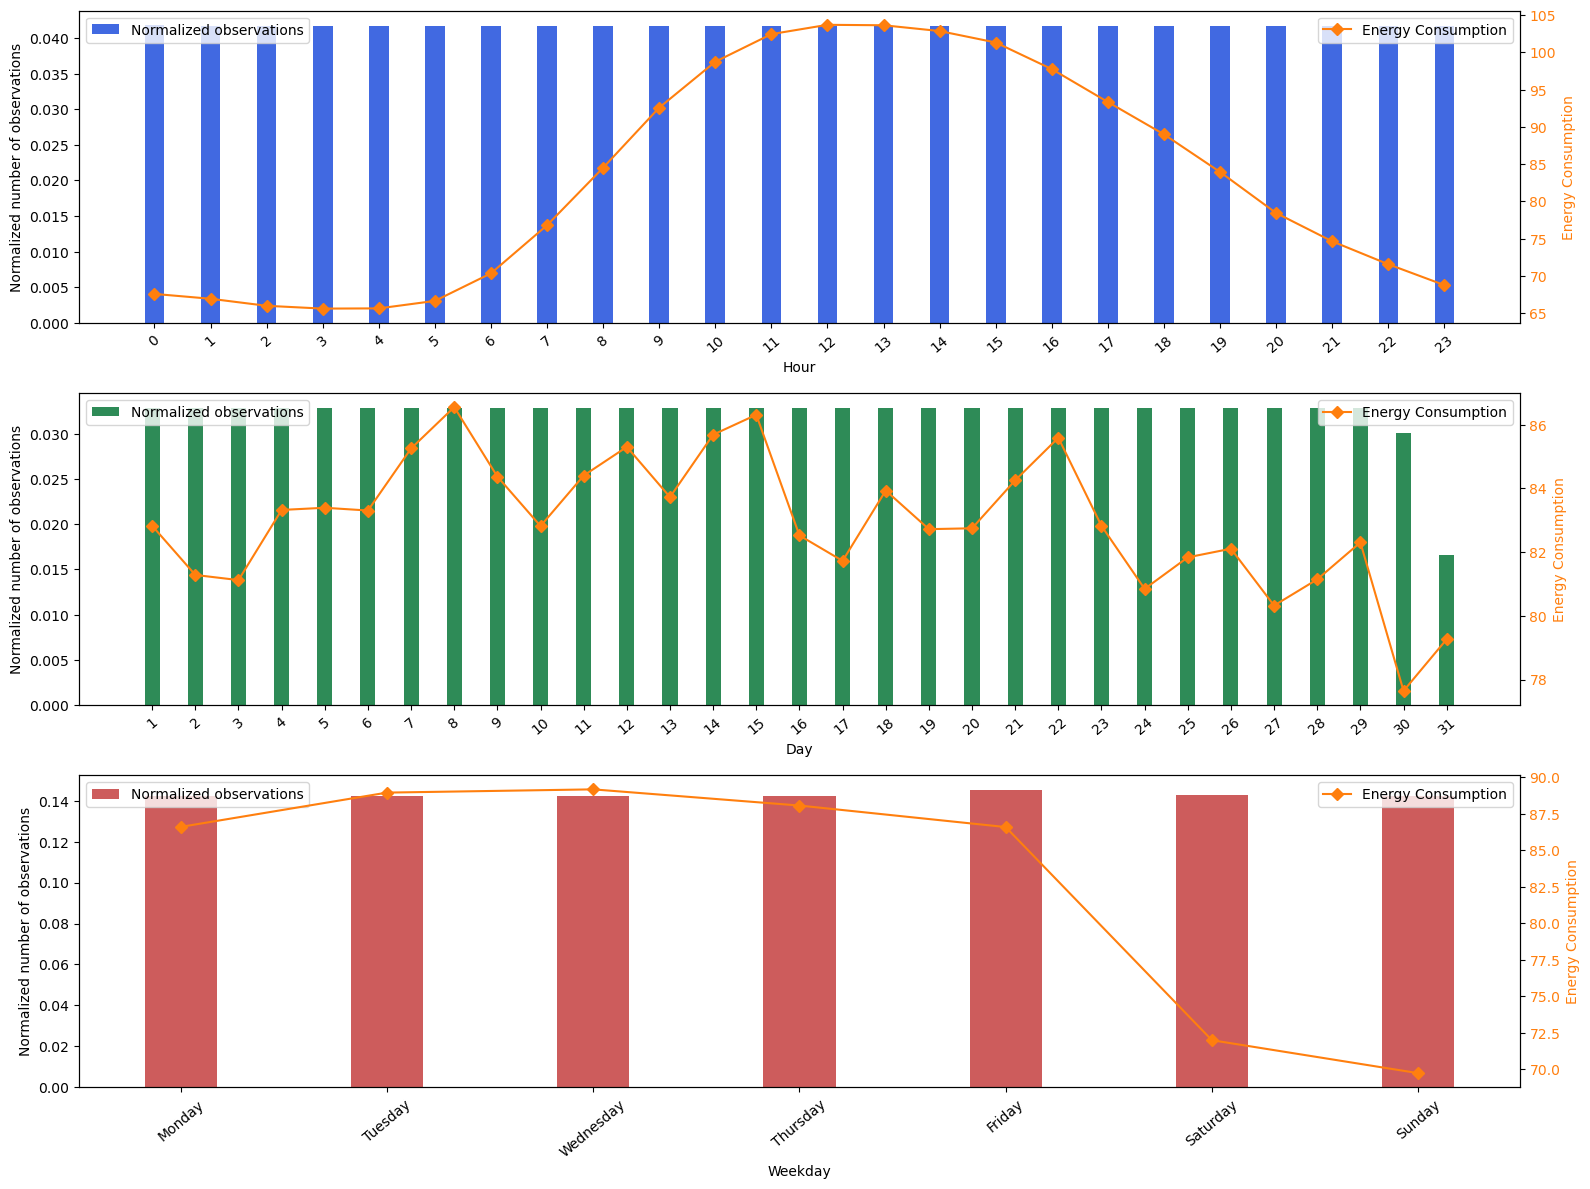
\includegraphics[width=1\linewidth]{images/avg_consumption_by_hour.png} \caption{Average energy consumption by hour of the day (across all buildings)} \label{fig:AvgConsumptionByHour} \end{figure}

\begin{figure}[!h] \centering 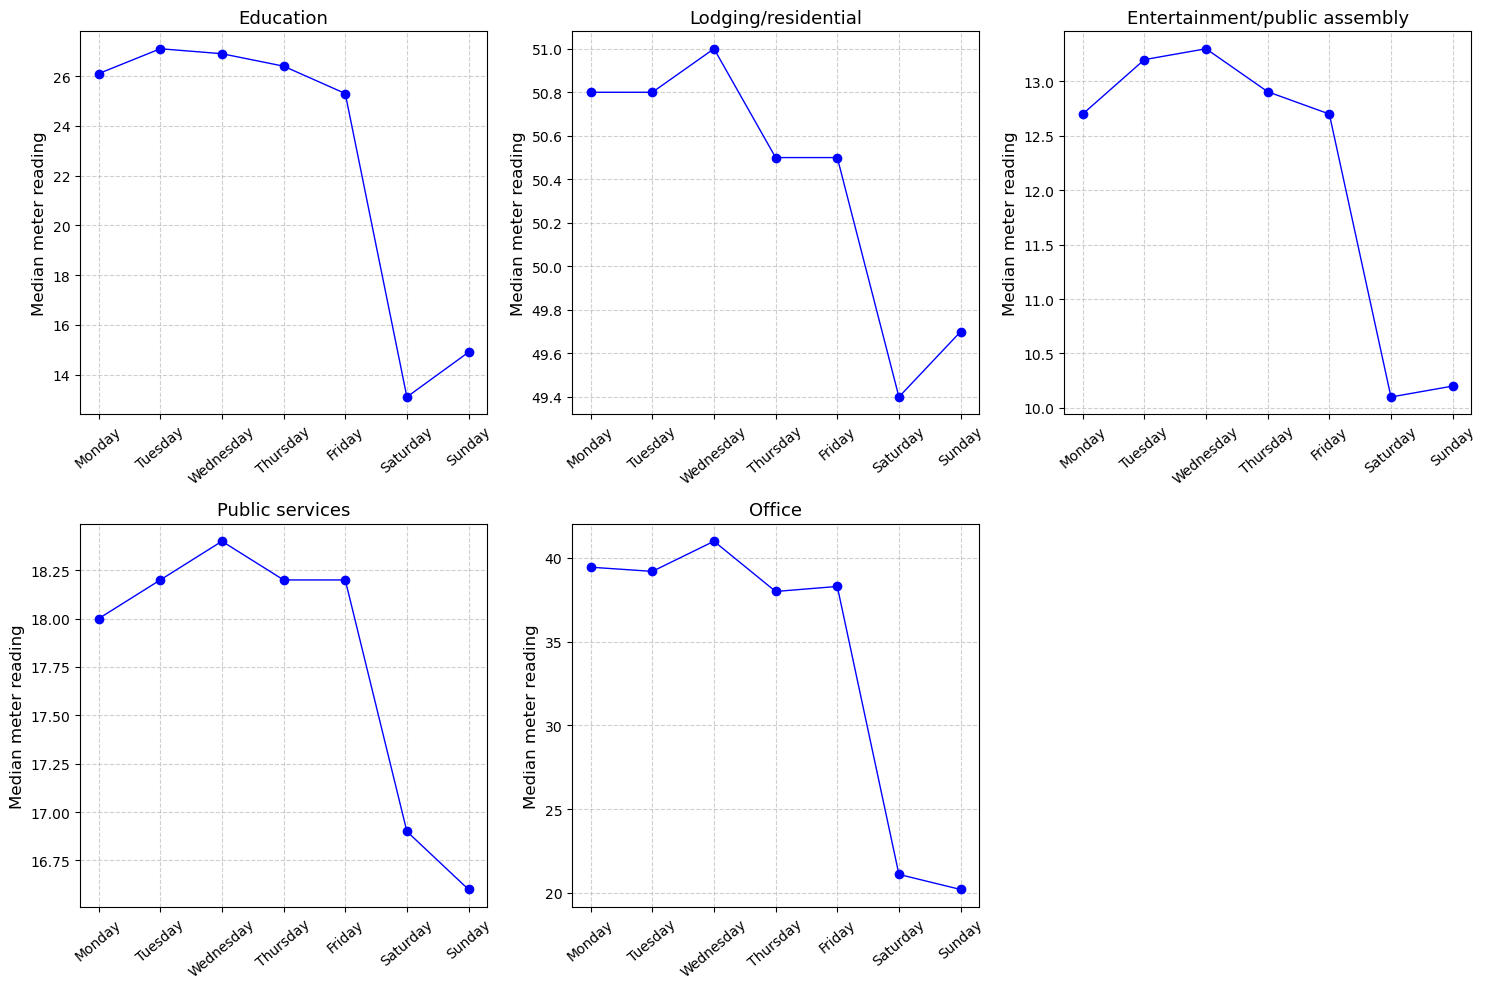
\includegraphics[width=1\linewidth]{images/primary_use_weekly_patterns.png} \caption{Weekly average consumption by primary use category} \label{fig:WeeklyByPrimaryUse} \end{figure}
\begin{figure}[!h] \centering 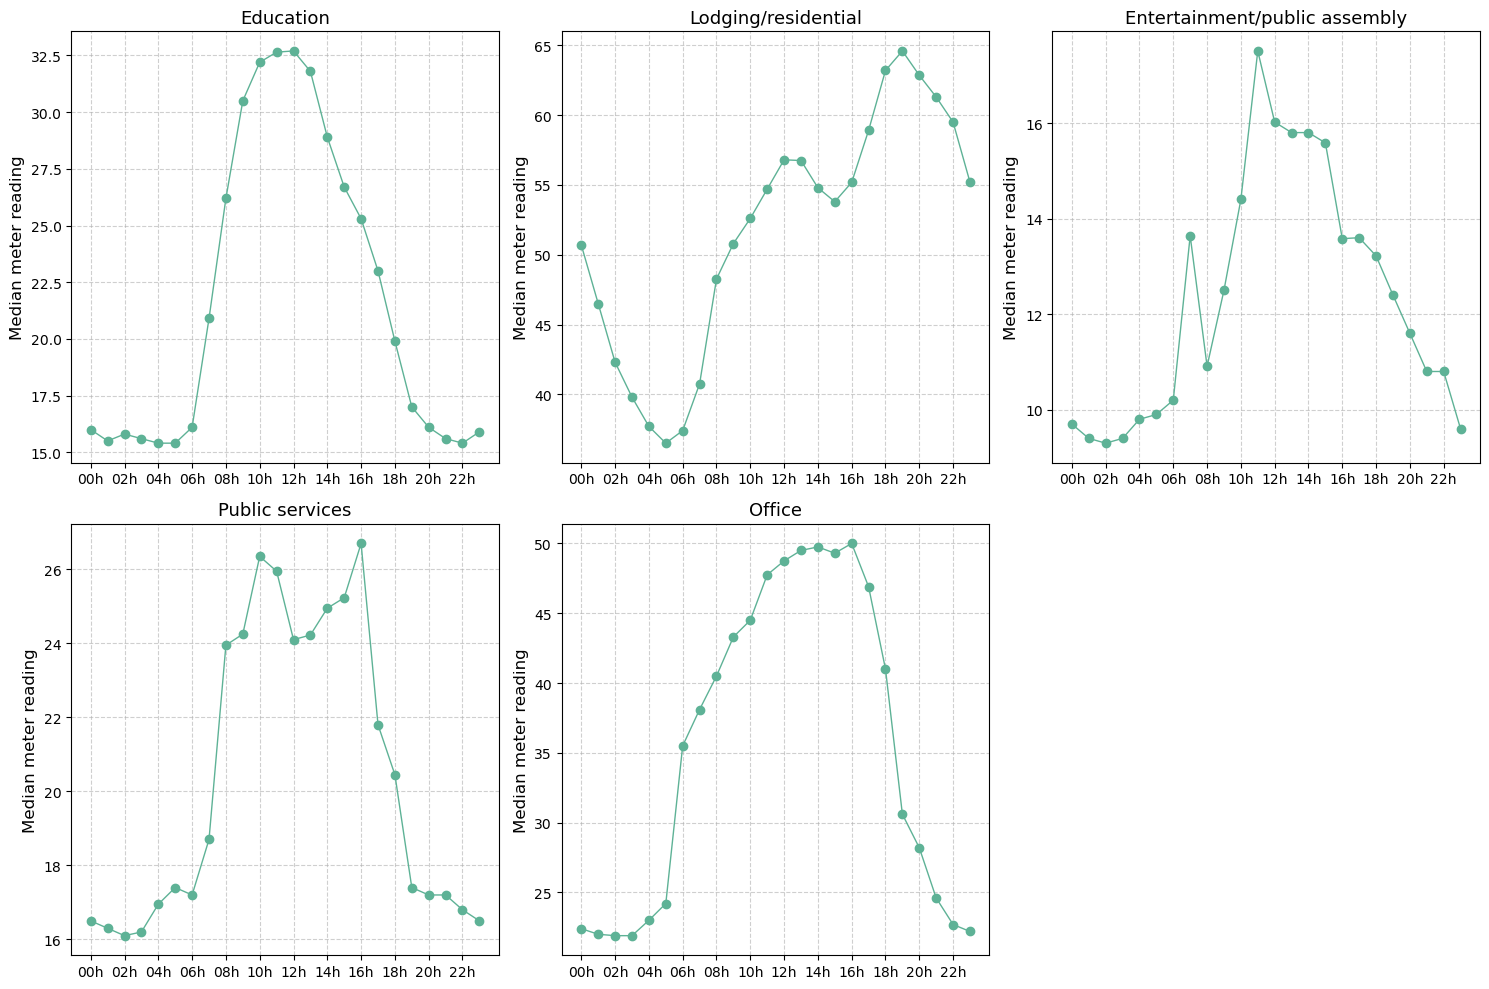
\includegraphics[width=1\linewidth]{images/primary_use_hours_patterns.png} \caption{Hours average consumption by primary use category} \label{fig:HoursByPrimaryUse} \end{figure}

To dig deeper, we disaggregated the data by primary\_use and analyzed the consumption behavior per category throughout the week, Fig. \ref{fig:WeeklyByPrimaryUse} and Fig. \ref{fig:HoursByPrimaryUse}. This comparison made clear that buildings categorized under Education, Public Services, Office, and Entertainment exhibit strong weekday-oriented consumption patterns, with peaks occurring between Monday and Friday from 8 am to 6 pm, and a sharp decline during weekends. These buildings typically operate on fixed schedules and are either closed or underutilized during the weekend.

On the other hand, Residential buildings (e.g., Lodging/Residential) display a different pattern: their energy consumption is more evenly distributed across the week, with subtle peaks during early mornings and evenings — aligning with typical home usage behavior. This contrast highlights how consumption habits differ significantly depending on the building type and its operational hours.

These findings also suggest that the overall weekday consumption bias observed in the aggregate data is likely influenced by the overrepresentation of Education, Office, and Public buildings in the dataset, compared to residential ones.

By identifying these temporal usage patterns and distinguishing between building types, we laid the foundation for time-aware modeling strategies that consider cyclical consumption behaviors — a critical step in improving prediction accuracy and interpretability in energy forecasting tasks.